\section{Operating-Point Signature Experiment}
\label{sec:ei-x02}

\subsection{Reference Correction and Response Correction}
The stream bank already builds local predictors at estimated operating
points. A separate experiment tests why changing a reference alone may be
insufficient. It compares three response approximations with identical
observations, channels, timing, amplitude prior and inference horizon.
It is a controlled test of a mixed derivative, not another version of R11.

Let $\eta$ denote a scalar operating change and $a$ the signed load factor.
Central differences of complete nonlinear DAE trajectories give
\begin{align}
 D_i(\eta)&\simeq\frac{y_i(\eta,h)-y_i(\eta,-h)}{2h},\nonumber\\
 E_i&\simeq\frac{D_i(d)-D_i(-d)}{2d}.
 \label{eq:ei-mixed-response}
\end{align}
The event follows the same ON/OFF schedule in every derivative trajectory.
The fixed $Q_i^0$ is the coefficient of $a^2$, obtained from the centered
second difference divided by $2h^2$. After removing the frozen common
angle drift, the three predicted histories are
\begin{align}
 \mu_i^{\rm N}(a)&=y_0+aD_i^0+a^2Q_i^0,\nonumber\\
 \mu_i^{\rm R}(a)&=\mu_i^{\rm N}(a)+\widehat b,\nonumber\\
 \mu_i^{\rm E}(a)&=\mu_i^{\rm R}(a)+a\widehat\eta E_i.
 \label{eq:ei-three-predictions}
\end{align}
Both corrected variants use exactly the same prefix offset $\widehat b$.
This comparator corrects the measured PMU reference; it is not the separate
nonlinear AC hidden-state reconstruction algorithm in the historical study.
Only the last changes the event signature. The first two consequently
have identical incremental response models even when their absolute fits
differ. Context $\widehat\eta$ is estimated by generalized least squares
from the pre-event PMUs and the nominal context direction. No test context,
source or severity enters inference.

\begin{figure*}[t]\centering
\begin{tikzpicture}[font=\sffamily\scriptsize,>=Latex,
 b/.style={draw=black!45,rounded corners=2pt,align=left,text width=4.3cm,minimum height=1.0cm,inner sep=5pt},
 a/.style={->,draw=black!65,thick}]
\node[b,fill=accessblue!7] (prefix) at (5.2,0) {\textbf{Same pre-event PMUs}\\Estimate $\widehat\eta$ and offset $\widehat b$.\\Use only reports before 2.5 s.};
\node[b,fill=green!7] (dict) at (0,0) {\textbf{Separate physical dictionary}\\Complete DAE trajectories produce\\$D_i^0$, $Q_i^0$ and mixed derivative $E_i$.};
\node[b,fill=orange!9] (data) at (10.4,0) {\textbf{Same held-out observations}\\Four candidate loads; known ON/OFF.\\Truth is unavailable to inference.};
\node[b,fill=accessblue!5] (nom) at (0,-1.8) {\textbf{Nominal}\\$y_0+aD_i^0+a^2Q_i^0$};
\node[b,fill=green!5] (recent) at (5.2,-1.8) {\textbf{Recentered}\\Nominal prediction $+\widehat b$};
\node[b,fill=orange!6] (cond) at (10.4,-1.8) {\textbf{Conditioned}\\Recentered prediction $+a\widehat\eta E_i$};
\node[draw=black!40,rounded corners=2pt,text width=14.6cm,align=center,inner sep=5pt] (out) at (5.2,-3.4) {\textbf{Same inference and evaluation:} colored-instrument transform, amplitude integral and priors.\\Compare response error, source/presence decisions and severity; retain every test case.};
\draw[a] (dict)--(nom);\draw[a] (prefix)--(recent);
\draw[a] (nom)--(recent);\draw[a] (recent)--(cond);
\draw[a] (data.east)--++(.25,0)|-(out.east);
\draw[a] (nom.south)--(out.north west);\draw[a] (recent)--(out);\draw[a] (cond.south)--(out.north east);
\end{tikzpicture}
\caption{Executed signature ablation, separate from the stream algorithm
in Fig.~\ref{fig:joint-architecture}. The three variants share the data
and decision calculation; only reference and event-response terms differ.}
\label{fig:ei-architecture}\end{figure*}


\subsection{Test Cases and Decision Contract}
The frozen F01 plant supplies all trajectories. The scalar $\eta$ scales
PQ operating injections and active PV dispatch; feasible initialization
can change permitted operating setpoints, but not machine constants,
line impedances, ZIP fractions or the PMU model. Central event/context
steps are 0.005 and 0.01, with step-halving checks. Dictionary construction
uses \EIDictionaryCases{} trajectories. The test contains \EITestPhysical{}
physical cases: \EIEventPhysical{} load interventions and \EINormalPhysical{}
controls at operating changes $-3\%,-2\%,0,+2\%,+3\%$. Each load changes
P/Q together by $\pm0.1\%$ or $\pm1\%$ at BUS3, BUS7, BUS16 or BUS24.
None belongs to the prescribed voltage-measurement PMU set; the separate
oriented current-terminal assignments remain fixed.

Each case is one ten-second integration, with ON at 3 s, OFF at 6 s and
no state reset. The context fit ends at 2.5 s. Three frozen instrumental
noise seeds produce \EIObserved{} paired records. The nonlinear PMU
frequency/ROCOF operator runs before its archived instrumental noise is
added. Both corrected methods retain the same measured prefix, so an
advantage cannot arise from supplying one method a better initial reference.\AIDraftingCredit{}

This experiment supplies the load family and ON/OFF times. It estimates
source and continuous severity using the same bounded Gaussian prior and
amplitude-integrated likelihood in all three variants. The no-event
hypothesis is retained. The fixed colored-instrument transform is common;
plug-in prefix estimates and clipped noise still limit probability
calibration. Thus these decisions are not unknown-onset detector scores
and normal-window decisions are not continuous false-alarm rates.

\subsection{Response Error and Source Decisions}
% Transposed from the generated X02 table, without changing values.
\begin{table}[t]\centering\footnotesize\setlength{\tabcolsep}{3pt}
\caption{Controlled known-onset load test. Response error uses 80 physical cases; joint and source-only correctness use 240 noisy event records. Severity error is evaluated at the generating source. The 15 normal windows are not normal-hours exposure.}
\label{tab:ei-results}
\begin{tabular}{lrrr}\toprule
Measure & Nominal & Recentered & Conditioned\\\midrule
Response error (\%) & 1.25 & 1.25 & 0.0561\\
Joint correct & 114/240 & 240/240 & 240/240\\
Source-only correct & 114/240 & 240/240 & 240/240\\
Normal selections & 12/15 & 0/15 & 0/15\\
Severity error (\%) & 3.45 & 1.2 & 0.329\\
\bottomrule\end{tabular}\end{table}

Relative to recentering alone, the mixed term reduces mean incremental response error: the paired difference is -1.15 percentage points (95\% interval [-1.31, -1]). The corresponding joint-decision difference is 0 percentage points ([0, 0]), which does not establish a directional improvement in joint source decisions. The recentered and conditioned source decisions are already at the test ceiling. Median absolute relative severity error, evaluated at the generating source, changes from 1.2\% to 0.329\%. Its mean paired change is -0.738 percentage points ([-0.898, -0.582]). Both variants select the correct source in every tested event record, so this severity comparison does not discard source errors. Their source masses numerically saturate at one; zero recorded log-loss is not evidence of calibrated uncertainty.


The gain is not uniform across all comparisons: at the nominal operating
point, estimating an unnecessary reference/context can worsen severity
relative to keeping the correct fixed reference. Figure~\ref{fig:ei-comparison}
retains that case rather than reporting only shifted operation.

The derivative stability checks change $E_i$ by
\EIContextFDLow{}--\EIContextFDHigh{}\% when the
context step is halved. Halving the event step in the two checked directions
changes it by at most \EIEventFDHigh{}\%. These are local numerical checks, not a
global smoothness or identifiability certificate.
Percentages of event severity refer to the P/Q input factors; actual load
power also responds to voltage under the frozen impedance law.

\begin{figure*}[t]\centering
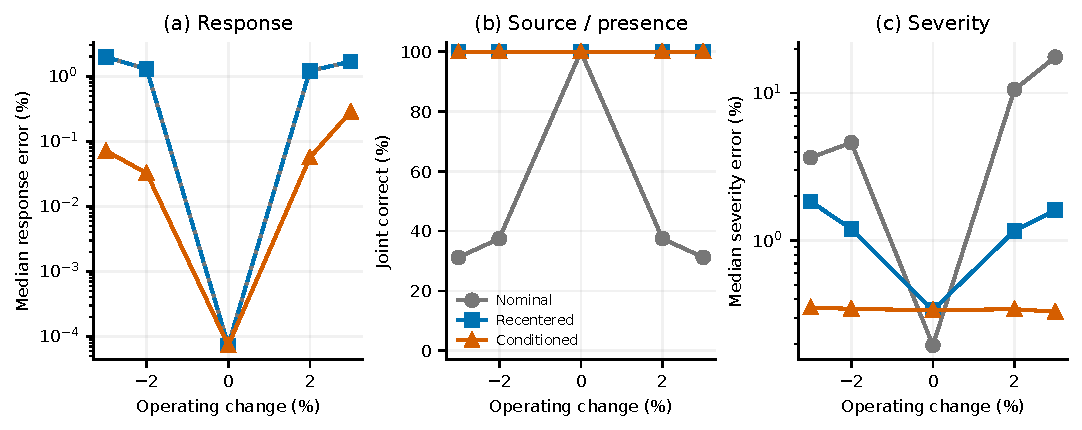
\includegraphics[width=.96\textwidth]{figures/generated/ei_x02_comparison.pdf}
\caption{Separate effects of recentering and conditioning. (a) Incremental
response error in the fixed physical test cases, evaluated at the generating
source and severity to isolate approximation error. (b) Correct source
and presence decisions on noisy observations, after marginalizing severity.
(c) Relative severity error evaluated at the generating source.
The panels measure different outcomes. Noise realizations repeat
physical cases and are not counted as additional independent trajectories.
Nominal and recentered incremental predictions coincide.}
\label{fig:ei-comparison}\end{figure*}

\begin{figure*}[t]\centering
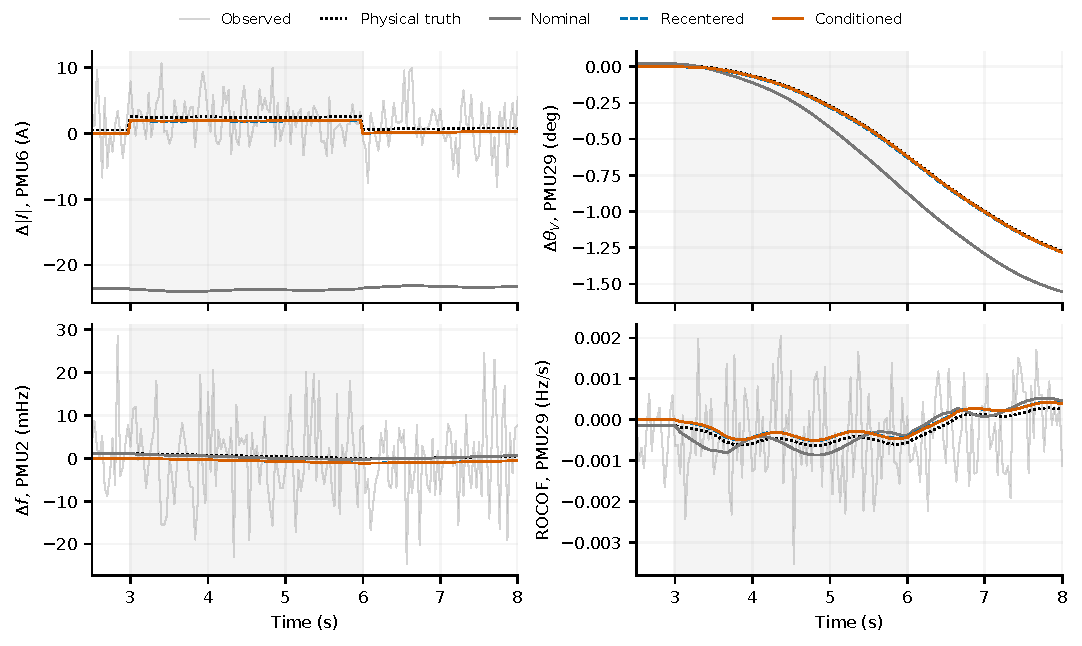
\includegraphics[width=.96\textwidth]{figures/generated/ei_x02_signals.pdf}
\caption{Fixed illustrative test: BUS7, $\eta=+3\%$, load factor $+1\%$,
seed 390502. Gray traces are the delivered PMU observations. Colored curves
use each method's selected source and estimated severity; a no-event
selection keeps its baseline. The dotted black curve is physical truth,
used only for illustration. The plotted channels and case were fixed
without selecting the largest improvement. Shading marks physical ON/OFF
for evaluation.}
\label{fig:ei-signals}\end{figure*}

Paired intervals resample physical test cases, keeping their noise seeds
and methods together. The same three noise seeds are reused across cases;
these intervals describe case variation conditional on those common noise
realizations, not uncertainty over a noise population or transfer to arbitrary
sources or plants. The step-halving checks and all
case outcomes remain in the frozen artifact package. Better fidelity, if
observed, is not sufficient to establish calibrated source probabilities,
all-family diagnosis or a benefit in the unchanged causal campaign.
